% Polish, Not Provenance
% Build: pdflatex main.tex, twice (the bibliography is typed in by hand, so no BibTeX step).
% Tables in tables/ and figures in figures/ are produced by `python -m paper.make_tables`.
% TODO before submitting: set the author name and affiliation below, and \repo.

\documentclass[conference]{IEEEtran}
\IEEEoverridecommandlockouts

\usepackage[T1]{fontenc}
\usepackage{cite}
\usepackage{amsmath,amssymb,amsfonts}
\usepackage{graphicx}
\usepackage{textcomp}
\usepackage{xcolor}
\usepackage{booktabs}
\usepackage{array}
\usepackage{microtype}
\usepackage{balance}
\usepackage{tikz}
\usetikzlibrary{arrows.meta}
\usepackage{hyperref}

\graphicspath{{figures/}}

\definecolor{accentblue}{HTML}{2A78D6}
\definecolor{accentorange}{HTML}{EB6834}
\definecolor{deepblue}{HTML}{184F95}
\definecolor{inkgray}{HTML}{555555}
\hypersetup{colorlinks=true, linkcolor=deepblue, citecolor=deepblue, urlcolor=deepblue}

\newcommand{\repo}{\texttt{[repository URL]}}
\newcommand{\auc}{\textsc{auc}}
\newcommand{\fpr}{\textsc{fpr}}
\newcommand{\tpr}{\textsc{tpr}}

\begin{document}

\title{Polish, Not Provenance: Testing Open-Source AI-Text\\Detectors on Matched Human and AI Writing}

\author{\IEEEauthorblockN{Author Name}
\IEEEauthorblockA{\textit{The Haverford School}\\
Haverford, PA, USA}}

\maketitle

\begin{figure*}[t]
\centering
\resizebox{\textwidth}{!}{%
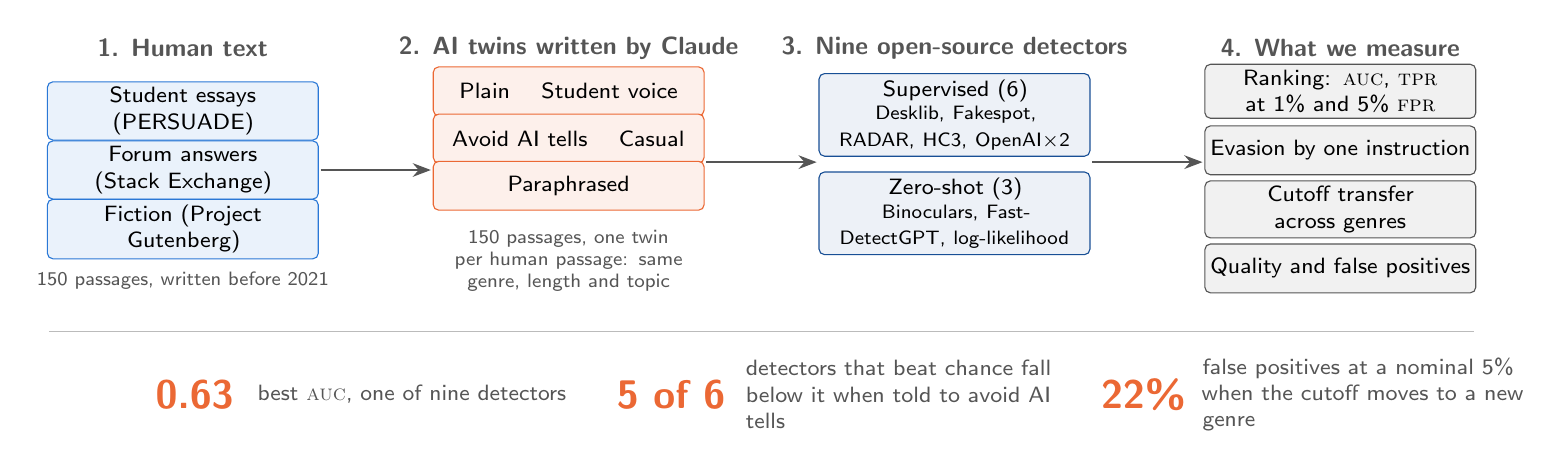
\begin{tikzpicture}[
    font=\sffamily\footnotesize,
    box/.style={draw=inkgray!70, rounded corners=2pt, fill=white, minimum height=0.62cm, text width=3.3cm, align=center, inner sep=2pt},
    hum/.style={box, draw=accentblue, fill=accentblue!10},
    ai/.style={box, draw=accentorange, fill=accentorange!10},
    det/.style={box, draw=deepblue, fill=deepblue!8, minimum height=1.05cm},
    metric/.style={box, draw=inkgray, fill=inkgray!8},
    head/.style={font=\sffamily\small\bfseries, text=inkgray},
    arr/.style={-{Stealth[length=2.3mm]}, line width=0.9pt, draw=inkgray},
    stat/.style={font=\sffamily\bfseries\Large, text=accentorange},
    statlabel/.style={font=\sffamily\footnotesize, text=inkgray, text width=4.1cm, align=left}
]
\node[head] at (0,2.35) {1. Human text};
\node[hum] at (0,1.55) {Student essays (PERSUADE)};
\node[hum] at (0,0.8)  {Forum answers (Stack Exchange)};
\node[hum] at (0,0.05) {Fiction (Project Gutenberg)};
\node[font=\sffamily\scriptsize, text=inkgray] at (0,-0.6) {150 passages, written before 2021};

\node[head] at (4.9,2.35) {2. AI twins written by Claude};
\node[ai] at (4.9,1.8)  {Plain \quad Student voice};
\node[ai] at (4.9,1.2)  {Avoid AI tells \quad Casual};
\node[ai] at (4.9,0.6)  {Paraphrased};
\node[font=\sffamily\scriptsize, text=inkgray, text width=3.4cm, align=center] at (4.9,-0.35) {150 passages, one twin per human passage: same genre, length and topic};

\node[head] at (9.8,2.35) {3. Nine open-source detectors};
\node[det] at (9.8,1.5)  {Supervised (6)\\[-1pt]\scriptsize Desklib, Fakespot, RADAR, HC3, OpenAI$\times$2};
\node[det] at (9.8,0.25) {Zero-shot (3)\\[-1pt]\scriptsize Binoculars, Fast-DetectGPT, log-likelihood};

\node[head] at (14.7,2.35) {4. What we measure};
\node[metric] at (14.7,1.8)  {Ranking: \auc, \tpr\ at 1\% and 5\% \fpr};
\node[metric] at (14.7,1.05) {Evasion by one instruction};
\node[metric] at (14.7,0.3)  {Cutoff transfer across genres};
\node[metric] at (14.7,-0.45) {Quality and false positives};

\draw[arr] (1.75,0.8) -- (3.15,0.8);
\draw[arr] (6.65,0.9) -- (8.05,0.9);
\draw[arr] (11.55,0.9) -- (12.95,0.9);

\draw[inkgray!40, line width=0.5pt] (-1.7,-1.25) -- (16.4,-1.25);
\node[stat] at (0.15,-2.05) {0.63};
\node[statlabel] at (3.0,-2.05) {best \auc, one of nine detectors};
\node[stat] at (6.2,-2.05) {5 of 6};
\node[statlabel] at (9.2,-2.05) {detectors that beat chance fall below it when told to avoid AI tells};
\node[stat] at (12.2,-2.05) {22\%};
\node[statlabel] at (15.0,-2.05) {false positives at a nominal 5\% when the cutoff moves to a new genre};
\end{tikzpicture}}
\caption{Study design. Each AI passage is a twin of one human passage and was written by Claude in one of five styles. Nine open-source detectors score every passage; we measure ranking quality, evasion by instruction, cutoff transfer across genres, and what gets flagged among human writing. Headline numbers are from Sections~\ref{sec:overall}--\ref{sec:domain}.}
\label{fig:design}
\end{figure*}

\begin{abstract}
Free AI-text detectors are used to judge student writing, but most evaluations test them on the kind of text they were trained on. We ask how nine open-source detectors, six supervised and three zero-shot, behave when human and AI text are matched in genre, length and topic, and when the AI is told how to write. We build a corpus of 150 human passages (student essays, forum answers, fiction), each paired with a twin written by Claude in one of five styles, plus three probe sets. The best detector, Desklib DeBERTa-v3-large, reaches an \auc\ of 0.63 (95\% CI 0.56--0.70) and catches 28\% of AI passages at a 5\% false positive rate; RADAR and two GPT-2-era detectors rank AI text below human text. A single instruction to avoid AI tells pushes five of the six detectors that beat chance on plain AI text below chance. Detection works on student essays (\auc\ up to 0.96 on plainly prompted AI essays) and mostly fails on forum answers and fiction, and cutoffs tuned on two genres misfire on the third (up to 22\% false positives at a nominal 5\%). Among human essays, better writing scores as more AI-like for three detectors (Spearman up to 0.42), which may be why English-learner essays were not flagged more often. These results suggest that current open-source detectors measure how polished and predictable writing is, not who wrote it.
\end{abstract}

\begin{IEEEkeywords}
AI-generated text detection, robustness, evasion, domain shift, academic integrity, false positives
\end{IEEEkeywords}

\section{Introduction}
Detectors for AI-written text are used by some schools to judge student work. A detector that falsely accuses a student of using AI has real costs, so the number that matters in practice is not overall accuracy but how much AI text a detector catches while it wrongly flags only a small share of human writing. Many free detectors exist, and many evaluations of them test text that resembles their training data, at the detector's default threshold, with AI text produced by a plain prompt.

That leaves four questions mostly unanswered. First, how well do detectors work when the human and AI passages are matched in genre, length and topic, so that none of these can be the signal? Second, what happens when the AI is simply told how to write: to sound like a student, to avoid sounding like AI, to write quickly and sloppily? Third, does a cutoff chosen on one kind of writing carry over to another? Fourth, among human text, what do the false positives have in common?

We answer these with a matched-twin design (Fig.~\ref{fig:design}). Each of 150 human passages (student essays, forum answers and fiction, all written before 2021) has an AI twin written by Claude to match its subject, length and position in its document, in one of five styles. We score all 300 passages, plus three probe sets, with nine open-source detectors. Our contributions are:
(i) a corpus design that pairs human and AI passages and varies only the instruction given to the AI, with per-passage instruction records;
(ii) a controlled evaluation of nine open-source detectors with confidence intervals that resample whole source documents and multiple-comparison correction;
(iii) evidence that a one-sentence instruction and a change of genre each break most detectors, and that false-positive-rate cutoffs do not transfer between genres; and
(iv) a human-side analysis showing that, within a prompt, better human essays score as more AI-like, and that English-learner essays are not flagged more often.

The strongest detector, Desklib DeBERTa-v3-large, reaches an \auc\ of 0.63 and catches 28\% of AI passages at a 5\% false positive rate. Three detectors are significantly backwards. Telling the model to avoid AI tells takes five of the six detectors that beat chance on plain AI text below chance. Only student essays are detected reliably.

\section{Related Work}
\textit{Zero-shot detectors} score text with a language model and need no labeled data. GLTR visualizes how predictable each token is \cite{gltr}. DetectGPT compares a passage's likelihood with that of perturbed versions \cite{detectgpt}, and Fast-DetectGPT replaces the perturbations with an analytic expectation over the model's own next-token distributions \cite{fastdetectgpt}. Binoculars divides a model's perplexity by the cross-perplexity between two related models \cite{binoculars}.

\textit{Supervised detectors} fine-tune a classifier on labeled human and AI text. OpenAI released a RoBERTa detector for GPT-2 output \cite{solaiman}. The HC3 corpus trained a RoBERTa detector on ChatGPT answers \cite{hc3}. RADAR trains a detector against a paraphraser so that it resists paraphrased AI text \cite{radar}. The RAID benchmark spans many generators, domains and adversarial attacks \cite{raid}, and the Desklib detector was trained on it \cite{desklib}.

\textit{Robustness and bias.} Paraphrasing evades many detectors \cite{krishna}, and theory suggests reliable detection becomes hard as models improve \cite{sadasivan}. RAID reports that detectors are brittle under adversarial attacks and across domains and generators \cite{raid}. Liang et al.\ found that GPT detectors flag essays by non-native English writers as AI \cite{liang}.

We differ in three ways. We match human and AI passages one to one, so length, genre and topic cannot carry the result. We vary only the style instruction given to the AI, which isolates evasion by instruction from evasion by editing tools. And we study the human side directly, with a quality score for each human essay.

\section{Corpus}
\label{sec:corpus}
\subsection{Human passages}
We collect human text from three open sources, all written before 2021: Stack Exchange answers (CC BY-SA) from ten non-programming sites, selected to have 5 to 40 votes and no edits after 2020; public-domain fiction from Project Gutenberg, one book per author with authors born in 1840 or later, skipping the first 15\% and last 10\% of each text; and student essays from PERSUADE 2.0 \cite{persuade}, written by US students in grades 6 to 12, with anonymization placeholders excluded. We take 50 passages from each source, cut at sentence boundaries to roughly 80 to 380 words, and normalize quotation marks and whitespace identically for human and AI text. Source, license, URL and date for every passage are recorded.

\subsection{AI passages}
Each AI passage was written directly by Claude \cite{claude}. No API pipeline, local model or script produced any text; every passage is a file a model wrote by hand after reading its instruction, which we log. The 156 non-paraphrase passages were written by Claude Fable 5.2 in six parallel writing sessions of about 26 passages each. The 24 paraphrases were written afterwards by Claude Sonnet 5.5, so they come from a different model than the passages they paraphrase. Three of the six sessions hit a usage limit after saving all their files but before reporting; we checked their lengths and shortened six overlong passages by deleting sentences by hand.

Every AI passage is the \emph{twin} of one human passage: the instruction gives the twin's title, its target word count, and where in its document the excerpt sits, and forbids reusing its wording. Written lengths ranged from 0.92 to 1.09 times target (mean ratio by style 0.99 to 1.05). There are five styles (Table~\ref{tab:styles}).

\begin{table}[t]
\caption{Instruction styles for the 150 main AI passages.}
\label{tab:styles}
\centering
\footnotesize
\begin{tabular}{@{}lp{5.1cm}r@{}}
\toprule
Style & Instruction (abridged) & $n$ \\
\midrule
Plain & none; write it naturally & 54 \\
Student voice & write like an ordinary US high school student & 24 \\
Avoid AI tells & no stock phrases, tidy lists or hedging; vary sentence length & 24 \\
Casual & fast and sloppy; typos and run-ons included & 24 \\
Paraphrased & reword an earlier plain passage, same content and length & 24 \\
\bottomrule
\end{tabular}
\end{table}

\subsection{Probe sets}
Three further sets address specific questions (Table~\ref{tab:corpus}). The \emph{English-learner probe} contains 50 PERSUADE essays by students marked as English language learners and 50 non-learner essays matched on prompt and grade. The \emph{imitation probe} pairs 30 real student essays with AI essays written to imitate each student's polish and mistakes. The \emph{essay-rewrite set} holds five student newspaper essays and AI rewrites of each at 25\%, 75\% and 100\% intended AI involvement, cut into 118 chunks of about 100 words. Its 25\% and 75\% versions are hybrids with no clean label, and its human essays date from 2024, so their label rests on the original authors' word and not on a date.

\begin{table}[t]
\caption{Corpus composition.}
\label{tab:corpus}
\centering
\footnotesize
\begin{tabular}{@{}lccp{2.9cm}@{}}
\toprule
Set & Human & AI & Used for \\
\midrule
Main & 150 & 150 & all primary results \\
English-learner & 100 & 0 & false positives \\
Imitation & 30 & 30 & imitating one student \\
Essay rewrites & 30 chunks & 88 chunks & partial AI use \\
\bottomrule
\end{tabular}
\end{table}

\subsection{Controls}
Word count alone separates the main human and AI sets with an \auc\ of 0.53 (95\% CI 0.46--0.60), so length is not a usable signal. Human fiction contains em dashes in 62\% of passages (Gutenberg writes dashes as double hyphens, which we converted) against 8\% of AI fiction; no detector's score differs detectably between human fiction passages with and without one.

\section{Detectors}
We test nine open-source detectors (Table~\ref{tab:detectors}), run locally on one laptop GPU. All scores are oriented so that higher means more AI-like. For every classifier we checked the AI class index against its authors' own code: RADAR's hosted demo reads the AI probability from output index 0, and OpenAI's server code unpacks its output as (fake, real).

\begin{table*}[t]
\caption{The nine detectors. S: supervised; Z: zero-shot.}
\label{tab:detectors}
\centering
\footnotesize
\begin{tabular}{@{}lclll@{}}
\toprule
Detector & Type & Backbone & Trained on & License \\
\midrule
Desklib \cite{desklib} & S, 2025 & DeBERTa-v3-L \cite{deberta} & RAID text \cite{raid} & MIT \\
Fakespot \cite{fakespot} & S, 2025 & RoBERTa-B \cite{roberta} & not listed & Apache-2.0 \\
RADAR \cite{radar} & S, 2023 & RoBERTa-L & Vicuna text, paraphraser & non-comm. \\
HC3 \cite{hc3} & S, 2023 & RoBERTa-B & ChatGPT answers & not stated \\
OpenAI-L \cite{solaiman} & S, 2019 & RoBERTa-L & GPT-2 samples & MIT \\
OpenAI-B \cite{solaiman} & S, 2019 & RoBERTa-B & GPT-2 samples & MIT \\
Binoculars \cite{binoculars} & Z, 2024 & Qwen2.5-1.5B pair \cite{qwen} & none & Apache-2.0 \\
Fast-DetectGPT \cite{fastdetectgpt} & Z, 2024 & GPT-Neo-2.7B \cite{gptneo} & none & MIT \\
Log-likelihood \cite{gltr} & Z, 2019 & GPT-Neo-2.7B & none & MIT \\
\bottomrule
\end{tabular}
\end{table*}

\textit{Zero-shot scores.} Let $p_\theta(v \mid x_{<t})$ be a model's next-token distribution. The log-likelihood score is the mean token log-probability. Fast-DetectGPT's analytic curvature compares the passage's total log-likelihood with its expectation under the model's own distributions, in units of the standard deviation of that expectation:
\begin{equation}
d(x)=\frac{\sum_t \log p_\theta(x_t \mid x_{<t})-\tilde\mu}{\tilde\sigma},
\end{equation}
where $\tilde\mu=\sum_t\sum_v p_\theta(v\mid x_{<t})\log p_\theta(v\mid x_{<t})$ and $\tilde\sigma^{2}=\sum_t \operatorname{Var}_{v\sim p_\theta(\cdot\mid x_{<t})}[\log p_\theta(v\mid x_{<t})]$.

Binoculars divides the log-perplexity under a performer model $M_2$ by the cross-perplexity between an observer $M_1$ and the performer:
\begin{equation}
B(x)=\frac{-\frac{1}{T}\sum_t \log p_{M_2}(x_t\mid x_{<t})}{-\frac{1}{T}\sum_t\sum_v p_{M_1}(v\mid x_{<t})\log p_{M_2}(v\mid x_{<t})}.
\end{equation}
Low $B$ indicates machine text, so we use $-B$. The original uses Falcon-7B and Falcon-7B-Instruct; those do not fit in the 12~GB of GPU memory we had, so ours uses Qwen2.5-1.5B and its instruct variant. It may be weaker than the published version for that reason alone. Both formulas are tested against hand calculations and against simulated text sampled from the scoring model.

\textit{Inputs.} Classifiers read up to 512 tokens (768 for Desklib), Binoculars up to 512, and the GPT-Neo scorers up to 1024; causal models run in half precision. Scoring all 578 texts with all nine detectors takes about six minutes. Model commit hashes are recorded with the scores.

\section{Evaluation Protocol}
Each detector's score is treated as a ranking; we do not assume it is a calibrated probability.

\textit{Metrics.} The main metric is the area under the ROC curve, the probability that a random AI passage outscores a random human one \cite{hanley}. Because falsely accusing a human is the costly error, we also report the true positive rate at a fixed false positive rate (1\% and 5\%), with the cutoff set from the human scores \cite{carlini}. Where a detector outputs a probability we also report a 0.5 cutoff.

\textit{Intervals and tests.} Passages from one source document are not independent, so intervals are 95\% percentile bootstrap intervals that resample whole documents \cite{efron,cameron}: a paraphrase moves with its source passage, and the five essays of the rewrite set resample as five units. Human and AI documents are resampled separately to keep group sizes fixed, with 2,000 resamples. P-values come from permutation tests with 10,000 shuffles of group labels between documents; paraphrases are compared with their sources by a paired sign-flip test, and rank correlations are tested by permuting within strata. We adjust with Holm's method \cite{holm} within each family of tests.

\textit{Cutoff transfer.} For each detector and each genre, we set the cutoff to allow 5\% false positives on the human text of the other two genres, and apply it to the held-out genre. If cutoffs carried over, the held-out false positive rate would stay near 5\%.

\textit{Human-side analyses.} We correlate each detector's score with the PERSUADE holistic quality score (1 to 6), by rank within prompt, over all 180 human PERSUADE essays in the corpus. We compare learners with non-learners both overall and within the same quality score.

\section{Results}
\subsection{Overall detection}
\label{sec:overall}
Table~\ref{tab:overall} and Fig.~\ref{fig:overview} summarize the nine detectors on the 150 human and 150 AI passages. Only Desklib is significantly above chance (\auc\ 0.63, Holm-adjusted $p=0.003$), and its lead over Fakespot is within noise (difference in \auc\ 0.06, 95\% CI $-0.02$ to 0.14). It catches 28\% of AI passages at 5\% false positives and 18\% at 1\%. Three detectors are significantly \emph{backwards}: RADAR (\auc\ 0.18), OpenAI-large (0.27) and OpenAI-base (0.38) rank AI text below human text. At a 0.5 cutoff RADAR flags 32\% of human passages and 2\% of AI passages, including 44\% of the real student essays and 48\% of the real forum answers. The 2019 detectors almost never flag the AI text, because it is nothing like GPT-2's.

Pairing each AI passage with its own human twin gives the same ranking: Desklib scored the AI twin higher in 70\% of pairs (95\% CI 62--78\%), RADAR in 11\% (6--17\%).

\begin{figure*}[t]
\centering
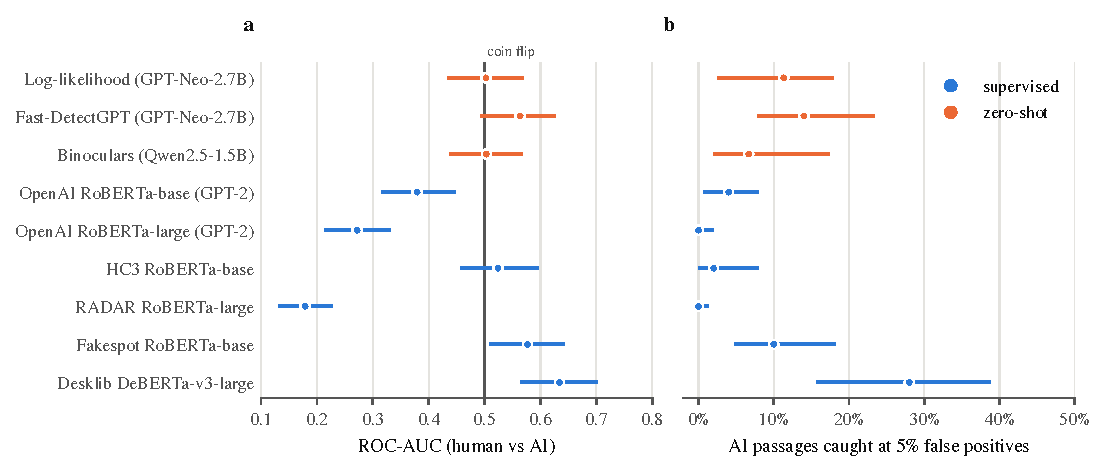
\includegraphics[width=\textwidth]{fig1_overview.pdf}
\caption{Nine detectors on 150 human and 150 AI passages. (a) ROC \auc\ with 95\% bootstrap intervals; the vertical line is a coin flip. (b) Share of AI passages caught when the cutoff allows 5\% of human passages through.}
\label{fig:overview}
\end{figure*}

\begin{table*}[t]
\caption{Detection on the main corpus (150 human, 150 AI). Brackets are 95\% document-level bootstrap intervals. The last column is the Holm-adjusted permutation $p$-value for \auc\ $\ne 0.5$. Best values in bold.}
\label{tab:overall}
\centering
\footnotesize
\begin{tabular}{@{}lcccc@{}}
\toprule
Detector & \auc\ [95\% CI] & \tpr\ at 5\% \fpr\ [95\% CI] & \tpr\ at 1\% \fpr & $p_{\text{Holm}}$ \\
\midrule
\multicolumn{5}{@{}l}{\textit{Supervised}} \\
Desklib DeBERTa-v3-large & \textbf{0.63 [0.56, 0.70]} & \textbf{28\% [16\%, 39\%]} & 18\% & 0.003 \\
Fakespot RoBERTa-base & 0.58 [0.51, 0.64] & 10\% [5\%, 18\%] & 7\% & 0.130 \\
RADAR RoBERTa-large & 0.18 [0.13, 0.23] & 0\% [0\%, 1\%] & 0\% & $<$0.001 \\
HC3 RoBERTa-base & 0.52 [0.46, 0.60] & 2\% [0\%, 8\%] & 1\% & 1.000 \\
OpenAI RoBERTa-large (GPT-2) & 0.27 [0.21, 0.33] & 0\% [0\%, 2\%] & 0\% & $<$0.001 \\
OpenAI RoBERTa-base (GPT-2) & 0.38 [0.32, 0.45] & 4\% [1\%, 8\%] & 2\% & 0.003 \\
\addlinespace
\multicolumn{5}{@{}l}{\textit{Zero-shot}} \\
Binoculars (Qwen2.5-1.5B) & 0.50 [0.44, 0.57] & 7\% [2\%, 17\%] & 3\% & 1.000 \\
Fast-DetectGPT (GPT-Neo-2.7B) & 0.56 [0.49, 0.63] & 14\% [8\%, 23\%] & 7\% & 0.279 \\
Log-likelihood (GPT-Neo-2.7B) & 0.50 [0.43, 0.57] & 11\% [3\%, 18\%] & 4\% & 1.000 \\
\bottomrule
\end{tabular}

\end{table*}

\subsection{One instruction changes the outcome}
\label{sec:evasion}
Fig.~\ref{fig:style} breaks the \auc\ down by how the AI passages were written, always against all 150 human passages. Six detectors beat chance on plain AI text: Desklib, Fakespot, HC3, Binoculars, Fast-DetectGPT and log-likelihood (\auc\ 0.61 to 0.72). For five of them, the instruction to avoid AI tells lowered the score significantly (Holm $p\le 0.005$) and sent the \auc\ below 0.5: Desklib falls from 0.67 (0.58--0.77) to 0.30 (0.20--0.41), Fakespot from 0.72 to 0.37, Binoculars from 0.61 to 0.22. At 5\% false positives, \emph{none} of the six catches a single one of the 24 avoid-tells passages. Asking for sloppy, casual writing has the same effect on Fakespot (0.72 to 0.35), HC3 (0.63 to 0.13) and log-likelihood (0.62 to 0.19), all with Holm $p=0.004$. Paraphrasing a plain passage lowers Fakespot's score in 18 of 24 pairs (Holm $p=0.038$), Fast-DetectGPT's in 21 of 24 and log-likelihood's in all 24 (both $p=0.004$); for Desklib, HC3 and Binoculars the paraphrase effect is not distinguishable from zero.

\begin{figure*}[t]
\centering
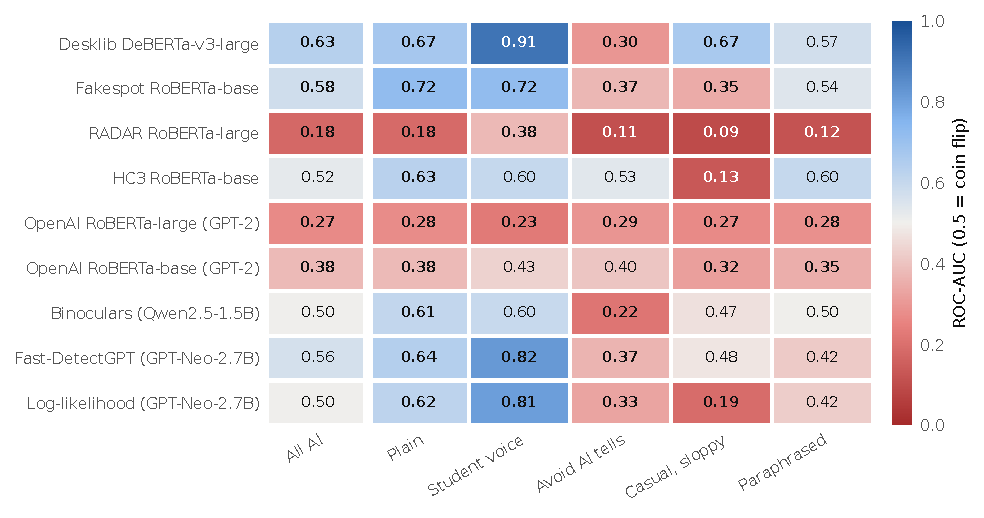
\includegraphics[width=0.72\textwidth]{fig2_style.pdf}
\caption{ROC \auc\ against all 150 human passages, by how the AI passages were written. Bold marks intervals that exclude 0.5. Blue: AI text ranks above human text. Red: below.}
\label{fig:style}
\end{figure*}

``Write like a high school student'' did not help the AI hide. For Fakespot the score is unchanged (Holm $p=1$), and for Desklib, Fast-DetectGPT and log-likelihood the student-voice passages scored higher than plain ones, so they were easier to catch (Desklib \auc\ 0.91, 0.85--0.96, catching 58\% at 5\% false positives), although none of those differences survives correction (smallest Holm $p=0.074$). Fig.~\ref{fig:percentile} shows the same effect on a common scale: each score is restated as the share of human passages scoring below it, so 0.95 is the 5\% false-positive cutoff for every detector.

\begin{figure*}[t]
\centering
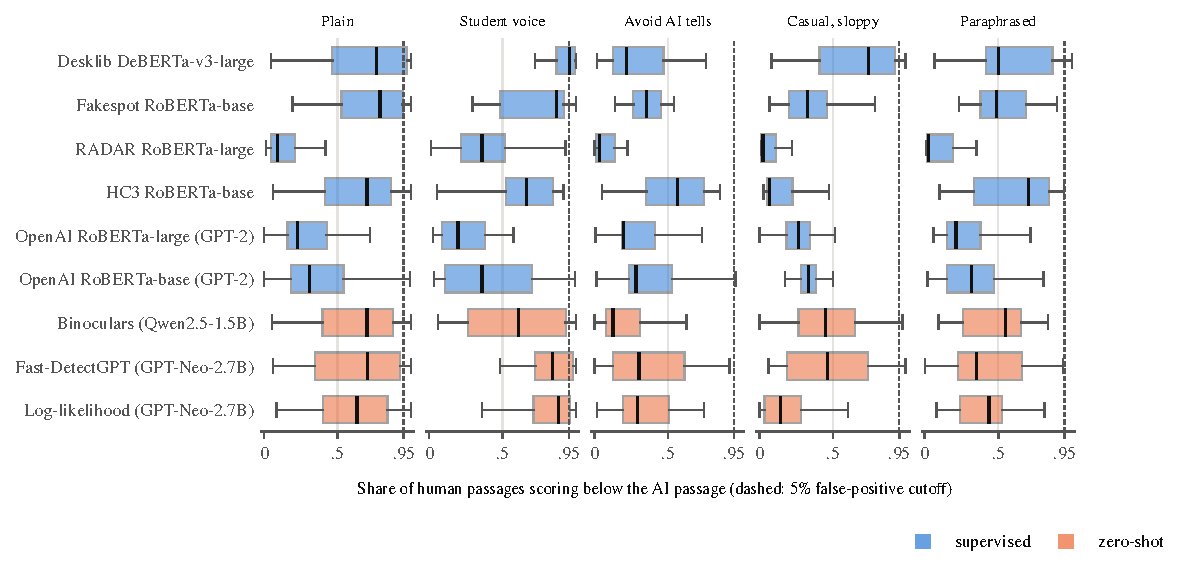
\includegraphics[width=\textwidth]{fig3_human_percentile.pdf}
\caption{Every AI passage's score restated as the share of the 150 human passages that score below it. The dashed line is the 5\% false-positive cutoff; a box left of it is mostly missed. Box: interquartile range; line: median.}
\label{fig:percentile}
\end{figure*}

\subsection{Domain shift and cutoff transfer}
\label{sec:domain}
Detection depends strongly on genre (Fig.~\ref{fig:genre}). On plainly prompted AI essays Desklib reaches an \auc\ of 0.96 (0.90--1.00) and catches 78\% at 5\% false positives, Fakespot 0.94 (0.88--0.98) and 56\%, and Binoculars, Fast-DetectGPT and log-likelihood 0.79 or better. On plainly prompted forum answers the best are Desklib (0.70) and Fakespot (0.66), and Fast-DetectGPT is backwards (0.25). On fiction only Fast-DetectGPT beats chance (0.76, catching 50\% at 5\% false positives). We suspect this reflects what the detectors were trained on, which we did not examine.

\begin{figure*}[t]
\centering
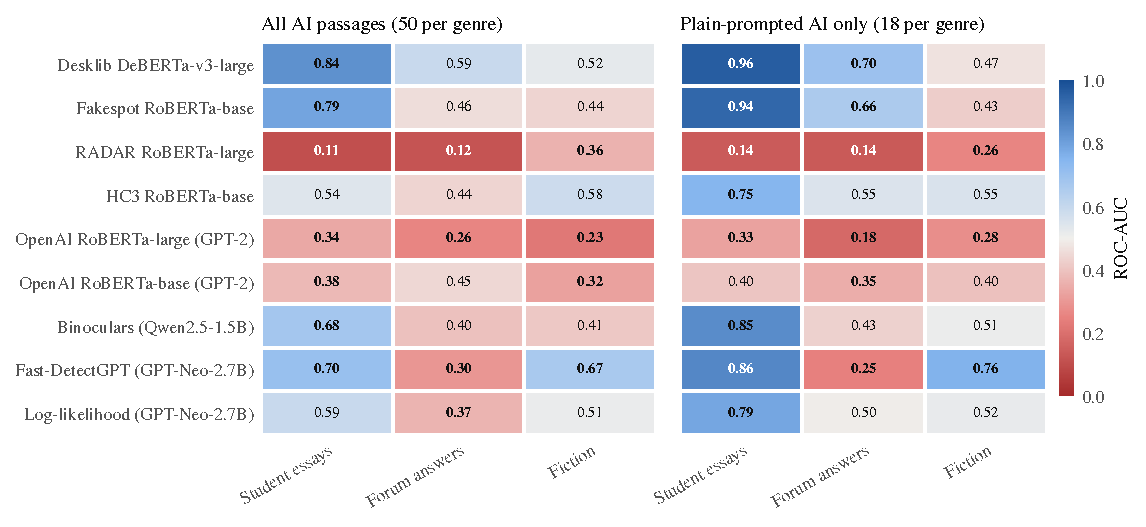
\includegraphics[width=0.86\textwidth]{fig4_genre.pdf}
\caption{ROC \auc\ by genre for all AI passages (left, 50 per genre) and plainly prompted AI only (right, 18 per genre). Rows are in the order of Fig.~\ref{fig:style}; bold marks intervals that exclude 0.5.}
\label{fig:genre}
\end{figure*}

A false-positive-rate cutoff also fails to travel (Fig.~\ref{fig:transfer}). With the cutoff chosen on forum answers and fiction, eight of nine detectors exceeded the 5\% target on student essays in their point estimates: Desklib 18\% (2--33\%), HC3 18\% (4--33\%) and log-likelihood 22\% (3--36\%) at the top. The opposite direction costs recall: with the cutoff transferred from forum answers and student essays, Desklib catches 4\% of the AI fiction, against 70\% of the AI student essays under the cutoff transferred to them.

\begin{figure*}[t]
\centering
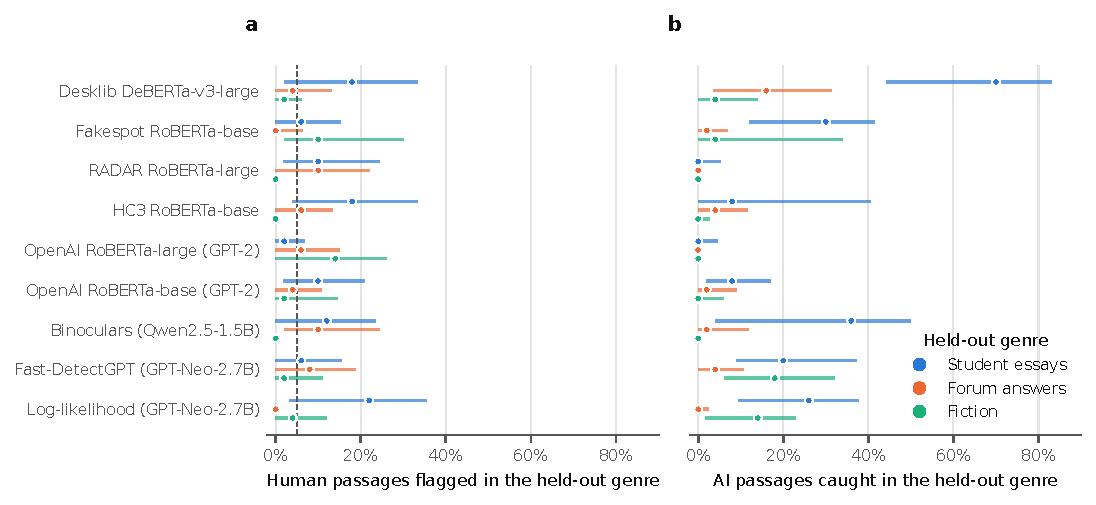
\includegraphics[width=\textwidth]{fig5_threshold_transfer.pdf}
\caption{Cutoff transfer. The cutoff allows 5\% false positives on the human text of the other two genres and is applied to the held-out genre. (a) False positive rate on the held-out genre's human passages; the dashed line is the 5\% target. (b) Share of that genre's AI passages caught. Bars are 95\% bootstrap intervals.}
\label{fig:transfer}
\end{figure*}

\subsection{What gets flagged among human writing}
\label{sec:human}
Within a prompt, better human essays score as more AI-like (Table~\ref{tab:humanside}, Fig.~\ref{fig:human}). Across the 180 human PERSUADE essays in the corpus, the rank correlation between holistic quality and detector score is 0.42 (0.29--0.53) for Fakespot, 0.39 (0.26--0.52) for log-likelihood and 0.34 (0.19--0.46) for HC3, all with Holm $p\approx 0.001$.

A familiar worry is that detectors flag non-native writers \cite{liang}. We did not see it. A learner essay outscored its matched non-learner essay only 24\% of the time for Fakespot (15--34\%, Holm $p=0.001$), and HC3, Binoculars and log-likelihood agree; Fakespot flagged 0\% of learner essays at 0.5 against 14\% of the others. The learner essays in this sample were rated lower (mean quality 2.4 against 3.5), so ``polish looks like AI'' and ``learners look more human'' may be one effect. Compared only within the same quality score, HC3's gap shrinks from 20 to 9 percentile points and is no longer significant, but Fakespot's stays at 25 (Holm $p=0.006$) and Binoculars' at 20 ($p=0.040$). A coarse 1-to-6 score cannot fully account for quality, so we do not claim it explains everything.

Surface features do not explain which human passages are flagged. We tested ten (length, sentence and word length, commas, contractions, first-person pronouns, quotation marks, digits, vocabulary variety) within genre; after correction only length survives, for two detectors: shorter human passages score higher with Desklib (rank correlation $-0.40$) and RADAR ($-0.51$).

\begin{figure*}[t]
\centering
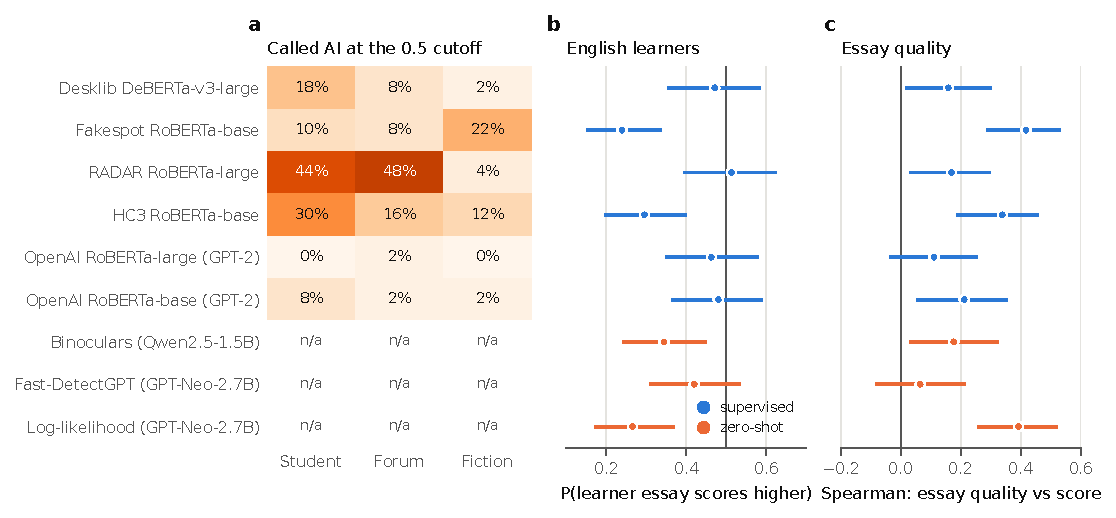
\includegraphics[width=\textwidth]{fig6_human_side.pdf}
\caption{Human-side results. (a) Share of human passages called AI at a 0.5 cutoff; zero-shot detectors have no such cutoff. (b) Probability that an English-learner essay scores higher than a non-learner essay on the same prompt and grade (0.5: no difference). (c) Rank correlation between a human essay's quality score and its detector score, within prompt.}
\label{fig:human}
\end{figure*}

\begin{table*}[t]
\caption{Human-written essays. Quality: Spearman correlation between holistic score and detector score, within prompt ($n=180$). Learners: probability that a learner essay outscores a matched non-learner essay ($n=50$ each). Matched gap: learner minus non-learner percentile-rank difference within the same quality score, in points. $p_{\text{Holm}}$ is for the matched gap.}
\label{tab:humanside}
\centering
\footnotesize
\begin{tabular}{@{}lcccc@{}}
\toprule
Detector & Quality $\rho$ [95\% CI] & Learners [95\% CI] & Matched gap & $p_{\text{Holm}}$ \\
\midrule
\multicolumn{5}{@{}l}{\textit{Supervised}} \\
Desklib DeBERTa-v3-large & 0.16 [0.02, 0.30] & 0.47 [0.35, 0.59] & $+$4 & 1.000 \\
Fakespot RoBERTa-base & 0.42 [0.29, 0.53] & 0.24 [0.15, 0.34] & $-$25 & 0.006 \\
RADAR RoBERTa-large & 0.17 [0.03, 0.30] & 0.51 [0.39, 0.63] & $+$5 & 1.000 \\
HC3 RoBERTa-base & 0.34 [0.19, 0.46] & 0.30 [0.20, 0.40] & $-$9 & 1.000 \\
OpenAI RoBERTa-large (GPT-2) & 0.11 [$-$0.04, 0.26] & 0.46 [0.35, 0.58] & $+$0 & 1.000 \\
OpenAI RoBERTa-base (GPT-2) & 0.21 [0.05, 0.35] & 0.48 [0.36, 0.59] & $-$6 & 1.000 \\
\addlinespace
\multicolumn{5}{@{}l}{\textit{Zero-shot}} \\
Binoculars (Qwen2.5-1.5B) & 0.18 [0.03, 0.33] & 0.34 [0.24, 0.45] & $-$20 & 0.040 \\
Fast-DetectGPT (GPT-Neo-2.7B) & 0.06 [$-$0.08, 0.22] & 0.42 [0.31, 0.54] & $-$9 & 1.000 \\
Log-likelihood (GPT-Neo-2.7B) & 0.39 [0.26, 0.52] & 0.27 [0.17, 0.37] & $-$17 & 0.057 \\
\bottomrule
\end{tabular}

\end{table*}

\subsection{Imitation and partial AI use}
\label{sec:partial}
When Claude imitated one specific student's polish and mistakes, three detectors still caught it: Desklib (\auc\ 0.86, 0.76--0.95), Binoculars (0.85, 0.75--0.93) and Fast-DetectGPT (0.85, 0.73--0.93), the last two catching 50\% at 5\% false positives; Fakespot did not (0.60, 0.44--0.73). Deliberately bad writing does not hide the AI from detectors that read predictability, and ``avoid the tells'' is a different instruction from ``write badly.''

On the essay-rewrite set (Table~\ref{tab:rewrites}) only Desklib and Fakespot can see the AI rewrites. Light AI editing is invisible (25\% versions: \auc\ 0.59 and 0.53), but an AI draft edited by a human (75\%) is detected (0.94 and 0.90). Their scores rise steadily with intended AI share (within-essay rank correlation 0.65 and 0.56, Holm $p=0.001$), while RADAR, HC3 and the OpenAI models trend the wrong way. Five essays is too few for the intervals to be reliable.

\begin{table}[t]
\caption{Essay-rewrite set: \auc\ of each AI version against the human originals, and the within-essay rank correlation between intended AI share and score.}
\label{tab:rewrites}
\centering
\footnotesize
\setlength{\tabcolsep}{3pt}
\begin{tabular}{@{}lcccc@{}}
\toprule
Detector & 25\% & 75\% & 100\% & $\rho$ \\
\midrule
\multicolumn{5}{@{}l}{\textit{Supervised}} \\
Desklib DeBERTa-v3-large & 0.59 & 0.94 & 0.93 & $+$0.65 \\
Fakespot RoBERTa-base & 0.53 & 0.90 & 0.87 & $+$0.56 \\
RADAR RoBERTa-large & 0.45 & 0.39 & 0.31 & $-$0.26 \\
HC3 RoBERTa-base & 0.38 & 0.38 & 0.24 & $-$0.42 \\
OpenAI RoBERTa-large (GPT-2) & 0.39 & 0.20 & 0.12 & $-$0.53 \\
OpenAI RoBERTa-base (GPT-2) & 0.39 & 0.22 & 0.17 & $-$0.44 \\
\addlinespace
\multicolumn{5}{@{}l}{\textit{Zero-shot}} \\
Binoculars (Qwen2.5-1.5B) & 0.45 & 0.44 & 0.41 & $-$0.15 \\
Fast-DetectGPT (GPT-Neo-2.7B) & 0.39 & 0.43 & 0.38 & $-$0.20 \\
Log-likelihood (GPT-Neo-2.7B) & 0.44 & 0.38 & 0.34 & $-$0.23 \\
\bottomrule
\end{tabular}

\end{table}

\subsection{Robustness checks}
AUC by writing session ranges from 0.57 to 0.70 for Desklib and from 0.50 to 0.64 for Fakespot, so no single session drives the results. The two zero-shot detectors built on one model correlate at 0.65, but Desklib correlates with the others at between $-0.10$ and 0.34, so the detectors are not measuring one thing.

\section{Discussion}
\textit{What the detectors seem to measure.} Detection works where the AI text is fluent, regular and polished, as in plainly prompted essays, and fails where it is told not to be. Among human essays, better writing scores higher. Together these point to polish and predictability as what the detectors respond to, not provenance. Instructions that reduce polish (casual) or predictability (avoid the tells) defeat them. We did not test this causal story directly and offer it as a hypothesis.

\textit{Backwards detectors.} RADAR and the two GPT-2 detectors are not weak so much as mismatched. The 2019 detectors learned artifacts of GPT-2 output, and recent chatbot text does not have them. RADAR was trained against paraphrased text from one model; we cannot tell whether its failure comes from Claude's writing being far from that model's or from its human training text (web pages) being far from forum answers, fiction and student essays.

\textit{Practical implications.} A detector's score should not be used as evidence against a student. Cutoffs set for a target false positive rate need to be set per genre and checked there, and detectors should be tested with evasion instructions, since a user can ask for them in one sentence. The one place a detector worked well, plain AI essays, is also the case where the author is least likely to have tried to hide anything.

\textit{Limitations.} All AI text comes from two models of one vendor, told to write in specific ways; their interpretation of ``sloppy'' and ``student'' is their own, and detectors tuned against other generators may behave differently. We cover three genres, with 150 passages per class and 24 per style, so style intervals are wide. We resample human and AI documents independently, which ignores the one-to-one matching. Percentile bootstrap intervals degrade when an estimate sits at zero (several catch rates are exactly 0\% with an interval of 0--0\%, meaning too small to measure). Holm correction is applied within each family of tests, and there are several families. PERSUADE's English-learner flag is coarse and self-reported, and its quality score runs from 1 to 6. We did not check publication years for each Gutenberg book. Our Binoculars is a smaller-model variant. Commercial detectors were out of scope, and nothing here says how they would do.

\textit{Future work.} The clearest next step is to repeat the quality analysis with a larger essay corpus and finer quality ratings, since it points to a mechanism. Adding several generators, humanizing tools and more genres, and testing per-genre cutoff calibration, would show whether the evasion and transfer results hold beyond this setting.

\section*{Statement on AI Assistance}
The AI passages in the corpus were written by Claude models, as described in Section~\ref{sec:corpus}. The analysis code, figures and a draft of this manuscript were also produced with assistance from Claude (Anthropic); the author is responsible for the content. Corpus, scores, result tables and code are available at \repo.

\balance
\begin{thebibliography}{99}

\bibitem{gltr} S. Gehrmann, H. Strobelt, and A. M. Rush, ``GLTR: Statistical detection and visualization of generated text,'' in \emph{Proc. 57th Annu. Meeting Assoc. Comput. Linguistics: System Demonstrations}, 2019, pp. 111--116.

\bibitem{detectgpt} E. Mitchell et al., ``DetectGPT: Zero-shot machine-generated text detection using probability curvature,'' in \emph{Proc. Int. Conf. Mach. Learn. (ICML)}, 2023.

\bibitem{fastdetectgpt} G. Bao et al., ``Fast-DetectGPT: Efficient zero-shot detection of machine-generated text via conditional probability curvature,'' in \emph{Proc. Int. Conf. Learn. Representations (ICLR)}, 2024.

\bibitem{binoculars} A. Hans et al., ``Spotting LLMs with Binoculars: Zero-shot detection of machine-generated text,'' in \emph{Proc. Int. Conf. Mach. Learn. (ICML)}, 2024.

\bibitem{solaiman} I. Solaiman et al., ``Release strategies and the social impacts of language models,'' \emph{arXiv preprint arXiv:1908.09203}, 2019.

\bibitem{hc3} B. Guo et al., ``How close is ChatGPT to human experts? Comparison corpus, evaluation, and detection,'' \emph{arXiv preprint arXiv:2301.07597}, 2023.

\bibitem{radar} X. Hu, P.-Y. Chen, and T.-Y. Ho, ``RADAR: Robust AI-text detection via adversarial learning,'' in \emph{Advances in Neural Information Processing Systems (NeurIPS)}, 2023.

\bibitem{raid} L. Dugan et al., ``RAID: A shared benchmark for robust evaluation of machine-generated text detectors,'' in \emph{Proc. 62nd Annu. Meeting Assoc. Comput. Linguistics (ACL)}, 2024.

\bibitem{desklib} Desklib, ``ai-text-detector-v1.01,'' Hugging Face model card, 2025. [Online]. Available: \url{https://huggingface.co/desklib/ai-text-detector-v1.01}

\bibitem{fakespot} Fakespot AI Labs, ``roberta-base-ai-text-detection-v1,'' Hugging Face model card, 2025. [Online]. Available: \url{https://huggingface.co/fakespot-ai/roberta-base-ai-text-detection-v1}

\bibitem{krishna} K. Krishna et al., ``Paraphrasing evades detectors of AI-generated text, but retrieval is an effective defense,'' in \emph{Advances in Neural Information Processing Systems (NeurIPS)}, 2023.

\bibitem{sadasivan} V. S. Sadasivan et al., ``Can AI-generated text be reliably detected?'' \emph{arXiv preprint arXiv:2303.11156}, 2023.

\bibitem{liang} W. Liang et al., ``GPT detectors are biased against non-native English writers,'' \emph{Patterns}, vol. 4, no. 7, 2023.

\bibitem{persuade} S. A. Crossley et al., ``A large-scale corpus for assessing written argumentation: PERSUADE 2.0,'' \emph{Assessing Writing}, vol. 61, 2024.

\bibitem{claude} Anthropic, ``Claude models.'' [Online]. Available: \url{https://www.anthropic.com}

\bibitem{roberta} Y. Liu et al., ``RoBERTa: A robustly optimized BERT pretraining approach,'' \emph{arXiv preprint arXiv:1907.11692}, 2019.

\bibitem{deberta} P. He, J. Gao, and W. Chen, ``DeBERTaV3: Improving DeBERTa using ELECTRA-style pre-training with gradient-disentangled embedding sharing,'' in \emph{Proc. Int. Conf. Learn. Representations (ICLR)}, 2023.

\bibitem{qwen} Qwen Team, ``Qwen2.5 technical report,'' \emph{arXiv preprint arXiv:2412.15115}, 2024.

\bibitem{gptneo} S. Black et al., ``GPT-Neo: Large scale autoregressive language modeling with Mesh-Tensorflow,'' Zenodo, 2021.

\bibitem{hanley} J. A. Hanley and B. J. McNeil, ``The meaning and use of the area under a receiver operating characteristic (ROC) curve,'' \emph{Radiology}, vol. 143, no. 1, pp. 29--36, 1982.

\bibitem{carlini} N. Carlini et al., ``Membership inference attacks from first principles,'' in \emph{Proc. IEEE Symp. Security and Privacy}, 2022.

\bibitem{efron} B. Efron, ``Bootstrap methods: Another look at the jackknife,'' \emph{Ann. Statist.}, vol. 7, no. 1, pp. 1--26, 1979.

\bibitem{cameron} A. C. Cameron, J. B. Gelbach, and D. L. Miller, ``Bootstrap-based improvements for inference with clustered errors,'' \emph{Rev. Econ. Statist.}, vol. 90, no. 3, pp. 414--427, 2008.

\bibitem{holm} S. Holm, ``A simple sequentially rejective multiple test procedure,'' \emph{Scand. J. Statist.}, vol. 6, no. 2, pp. 65--70, 1979.

\end{thebibliography}

\end{document}
